\chapter{螺旋线}
慢波系统是行波管的主要部件之一,它是管内传播高频电磁波的一种特殊传输线。按照在行波管中所起的作用,我们对慢波线提出了以下三个基本要求:一是能使高频电磁波的传播速度减慢,以便与电子流“同步”,进行充分的能量交换;二是要求慢电磁波的传播速度随频率的变化尽量小,这样,当不同频率的电磁波进入该慢波线时就都能与电子流“同步”,因而都能得到放大,行波管的频带就能做得很宽。讲到这里,读者也许要问:在第二章里不是说过传输线的频带是很宽吗?这里为什么又作为一条基本要求提出来呢?这是因为慢波线一般都不是均匀的传输线,我们知道,均匀传输线(如同轴电缆)的频带是非常宽的,而非均匀传输线的频带就要窄得多,非均匀传输线的频带宽度是与它们的不均匀程度有密切的关系的,不同的慢波线,由于其结构上的不同就会带来频带宽度的不同。因此,我们在设计慢波线的时候,很重要的一点就是要算出它的频带宽度是否能满足我们的要求。对于慢波线的第三个基本要求是希望在慢波线中电子注通过的地方能够建立起较强的轴向电场,这样,电子与高频电场之间才能产生有效的能量交换。

上一章中提到的螺旋线是一种能够较全面地满足上面三个基本要求的慢波线。特别是由于它具备了频带宽这样一条突出的优点,加上其结构简单、容易制作,所以中小功率行波管中几乎毫无例外地都采用螺旋线来作为它们的慢波系统。本章将对螺旋线的主要特效及若干实际问题作一简略介绍。
\section{螺旋线是怎样使电磁波速度变慢的?}
我们来看看图\ref{ch3-1}所示的一根用细金属丝绕成的螺旋线假定它的轴线与坐标轴$ Z $轴重合,平均直径等于$ 2a $,螺距等于$ p $,螺旋角(螺旋线上任意一点的切线与过该点所作$ Z $轴垂直平面之间的夹角称为螺旋角)等于$ \psi $。当电磁波以光速$ c $从螺旋线上的某点$ A $沿细金属丝传播到另一点$ B $时,如果$ B $点正好是沿金属丝绕行一圈到达的那个点,那么,电磁波沿金属丝所传播的距离可由图\ref{ch3-1}右边所示的一圈螺旋线的展开图上求得,它等于$\frac{2\pi a}{\cos \psi} $。但如果我们来观察同一时间内电磁波沿$ Z $轴的传播距离的话,它只前进了一个螺距$ p $。因此,电磁波沿$ Z $轴的传播速度$ v_p $与光速$ c $的比值等于:
\begin{equation}
	\frac{v_p}{c} = \frac{p}{\frac{2\pi a}{\cos \psi}} = \frac{p}{2\pi a}\cdot \cos\psi
\end{equation}
它反映了电磁波沿$ Z $轴的传播速度比光速减慢的程度,叫做螺旋线的“慢波比”。如果知道了电子注的运动速度$ v_0 $,那么就可以适当选择螺旋线的几何尺寸,使得$ v_p \approx v_0 $,即实现电磁波与电子注的“同步”。如前所述,在行波管实际工作时,为了达到真正的“同步”,通常还需要用改变螺旋线电压的办法来调节$ v_0 $,也就是进行“细调”。
\begin{figure}[phtb]
	\centering
	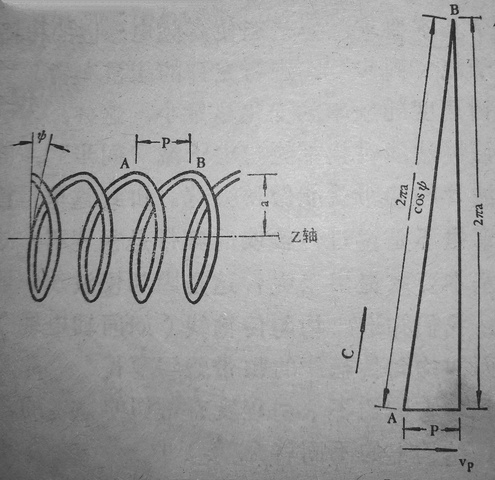
\includegraphics[width=0.65\linewidth]{figure/ch3-1}
	\caption{螺旋线的螺距、螺旋角和半径:$ \frac{v_p}{c} = \frac{p}{2\pi a} \cos \psi$}
	\label{ch3-1}
\end{figure}

上面的分析方法虽然便于直观地理解螺旋线中电磁波传播速度变慢的工作原理,但是,应该指出,这种分析是很粗略的。因此,它不能十分准确地反映实际情况。比如,由它似乎可以得出“慢电磁波的传播速度不随频率而变化”[因为式\ref{ch3-1}中不包含频率$ f $这样的错误结论。实践证明,对一个结构一定的螺旋线来说,虽然慢电磁波的传播速度在一定的频率范围内变化较小,但毕竟还是有变化的,这种变化对于行波管的工作是有影响的。因此,为了准确地设计螺旋线的结构,保证行波管的宽频带运用,就必须进一步研究慢电磁波的传播速度与频率之间的关系,即“色散特性”。


\section{色散特性}
慢电磁波的传播速度随频率而变化的情况,通常都用慢波系统的色散特性来表示。“色散”原是指光学中的一个物理现象。我们知道,光也是一种电磁波,只是它的频率要比微波高得多罢了。光因其频率的不同而呈现各种颜色,而白光则是由多种频率的单色光混合而成的。不同颜色的光在真空中传播时速度都是相同的,但是在介质(例如玻璃等)中传播时,它们的速度就随频率而不同了。因此,如果让不同颜色的光以同一个方向从空气中斜入射到玻璃介质中去,那么,由于折射角将随频率而变化,它们在玻璃中的传播方向就各不相同了。我们可以做一个实验来证实这个现象:让一束白光从空气中入射到玻璃棱镜中去,在玻璃棱镜的后面放置一个白色的屏幕,那么,白光中的各种单色光就将以不同的折射角从玻璃棱镜中射到白色屏幕上,于是,在白色屏幕上我们就可以看到依次排列的红、橙、黄、绿、青、兰、紫等各种颜色,这种现象便称为色散”。可见,色散的本质就是光在介质中的传播速度随频率而变化的特性。我们在描述慢波线中慢电磁波的传播速度随频率而变化的特性时,也采用了这个名称。

螺旋线的色散特性可以通过理论分析和实验测量两种途径得到。图\ref{ch3-2}所表示的螺旋线色散特性,就是在对实际螺旋线作了一定简化假设的条件下,用电磁场理论对电磁波沿螺旋线的传播规律进行数学分析后得出来的。图中纵坐标为$ \frac{v_p}{c} $,因为光速$ c $为常数,所以纵坐标的值是与$ v_p $正比的。横坐标为$ ka $其中$ a $是螺旋线的平均半径,对于结构已经确定的螺旋线来说,$ a $是一个常数。$ k=\frac{2\pi f}{c} $是电磁波在自由空间传播时的相位传播常数,它的物理意义将在后面介绍。由上可见,横坐标$ ka $是与频率$ f $成正比的。因此,图\ref{ch3-2}就表示了$ v_p $和$ f $的关系,也就是色散特性。
\begin{figure}[phtb]
	\centering
	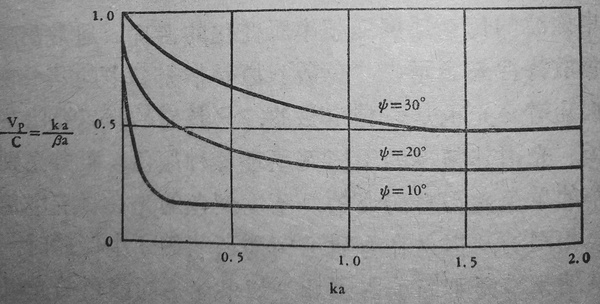
\includegraphics[width=0.65\linewidth]{figure/ch3-2}
	\caption{螺旋线的色散特性曲线}
	\label{ch3-2}
\end{figure}

从图\ref{ch3-2}的曲线中我们可以看到,当频率较高时,$ v_p $基本不变,且只与螺旋角$ \psi $有关。它的数值可以近似用$ \ref{ch3-1} $式算得,在$ \psi $较小的情况下,$ \ref{ch3-1} $式可以写成:
\begin{equation} \label{eq:ch3-2}
	\frac{v_p}{c}= \sin \psi \approx \tan\psi = \frac{p}{2\pi a}
\end{equation}
可以看出,\ref{eq:ch3-2}式是与上一章中的\ref{eq:ch2.1}式一致的。在实际的行波管中,工作频率不能任意提高,因为当频率超过一定范围后将会引起返波振荡(见第\ref{ch5}章),造成行波管工作的不稳定。为了避免返波振荡出现,通常在设计螺旋线时,总是使$ ka < 0.3 $。

我们在设计螺旋线型行波管时,常常是根据一定的原则先确定电子注电压(即螺旋线电压)$ U_0 $,从而也就决定了电子速度$ v_0 $和慢电磁波的传播速度$ v_p $。例如,微波通信设备所用的某中小功率行波管,其$ U_0 $为3千伏,对应的电子速度$ v_0 $约为光速$ c $的十分之一,由此可算得螺旋角约$ 6^\circ $。由图\ref{ch3-2}可见此时的色散特性曲线上有很宽的弱色散区(弱色散区是指$ v_p $随$ f $变化很小的区域,角越小,弱色散区越宽)。因此,尽管把$ ka $限制在0.3以下,由于$ U_0 $较低,$ \psi $较小,我们仍然可以得到很宽的频带。例如,对上例中$ \psi \approx 6 ^\circ $的情况,$ ka $只要大于$ 0.1 $左右,特性就很平了,如果$ a=1.5 $毫米,那么与$ 0.1<ka<0.3 $相对应的频率范围就是$ 3.2<f<9.5 $千兆赫,可见频带是很宽的。

慢波线的色散特性除了能够用$ \frac{v_p}{c}\textasciitilde ka$曲线直观地表示以外,还可以用所谓“$\omega -\beta $”曲线来表示,而且$ \omega-\beta $曲线能够更多地反映出慢波系统的主要特性。为了说明这个曲线,我们先来熟悉一下描述电磁波传播特性的几个基本量。



常数了。由$ \omega \textasciitilde \beta $曲线我们还可以确定慢波线的一些其它传播特性。例如曲线上任意一点的切线斜率就等于波的“群速”$ v_g $(即波的能量传播速度,它和波的相位传播速$ v_p $不同);由曲线的形状可以判断出$ v_g $和$ v_p $的符号是否相同,实际上就是群速和相速的方向是否相同?我们把$ v_g $和$ v_p $,方向相同的波称为“前向波”,而$ v_g $和$ v_p $方向相反的波则称为“返波”。正是由于$ \omega \textasciitilde \beta $曲线能够更多地表示出慢波线的传播特性,所以应用更为广泛。

关于波的群速、前向波与返波等问题,因超出了本书范围,这里不赘述。
\section{耦合阻抗}
耦合阻抗是表征慢波线中轴向高频电场与电子之间能量交换的有效程度的一个参量(用符号$ K_c $表示)。在螺旋线型行波管中,电子注是在螺旋线内沿着它的轴线方向运动的,因此,只有轴向高频电场才能和电子产生能量交换作用。当电磁波沿螺旋线向前传播时,它在电子注流过处(具体说来也就是螺旋线内半径为$ b $的细圆柱体内。$ b $是电子注半径)产生的轴向高频电场越强,那么电子与轴向高频电场的能量交换作用也越强。电子注流过处轴向高频电场的大小与螺旋线的结构有关,螺旋线结构不同时,它的高频场分布就不同,因此为了求出电子注流过处轴向高频电场的大小,就需要找到螺旋线的场分布,图\ref{ch3-5}表示了螺旋线周围的高频场分布。

电子注流过处轴向高频电场的大小还与螺旋线中传播的高频场功率有关。显而易见,送入螺旋线的高频场功率越大,那么它在电子注流过处产生的轴向高频电场也越强。为了便于对不同的螺旋线中电子与场能量交换的有效程度进行比较,我们希望能建立一个统一的衡量标准。首先,在不同的螺旋线中应该送入相同的高频场功率。在相同的高频场功率下,我们再来观察哪一种螺旋线所产生的轴向高频电场大,这样才能比较出哪一种螺旋线的相互作用有效程度强。这实际上就是希望在新导出的用来衡量相互作用有效程度的参量中去掉高频场功率带来的影响。从$\text{压强}= \frac{\text{压力}}{\text{受压面积}} $(即压强等于单位面积所受到的压力)这个公式我们联想到,这个新参量是否可以用送入单位功率所产生的轴向高频电场的大小来表示呢?根据这个想法并类比了低频电路的情况,人们导出了一个新的参量,这就是耦合阻抗$ K_c $。

我们知道,在低频电路中,当我们在谐振频率下往某一谐振回路中送入一定的功率$ P $时,在回路两端所产生的谐振电压振幅$ U $和回路的谐振电阻$ R $有下面的关系:
\begin{equation} \label{eq:ch3-17}
	R = \frac{1}{2}\frac{U^2}{P}
\end{equation}
回路的谐振电阻$ R $越大,那么其两端产生的谐振电压也越大因此$ R $是表征谐振回路特性的一个重要参量。

同样道理,我们把慢波系统的耦合阻抗$ K_c $定义为:
\begin{equation} \label{eq:ch3-18}
	K_c = \frac{1}{2}\frac{\hat{U_z^2}}{P}
\end{equation}
式中$ P $为沿螺旋线传播的高频场总功率。$ \hat{U_z} $为轴向高频电压的振幅,它是从低频电路的关系式\ref{eq:ch3-17}中类比得来的。我们知道,在微波频率下,通常只采用高频电场这个概念,例如我们常常用场强计来测量高频电场的大小,用功率计来测量高频场的功率大小,而从不用伏特计(电压表)来测量微波高频电场。因此,这里所说的轴向高频电压$ \hat{U_z} $是为了和低频电路类比而人为地导出来的一个量,不过,我们可以利用直流电路中电压和电场之间的关系把它和轴向高频电场$ \hat{E_z} $联系起来。我们知道,在均匀直流电场中,$ a $、$ b $两点之间的电压$ U_{ab} $可用电场$ E $和两点之间的距离$ d_{ab} $表示:
\begin{equation} \label{eq:ch3-19}
	U_{ab} = -E\cdot d_{ab}
\end{equation}
负号表示$ U $和$ E $的方向相反。如果不是均匀电场,那么,可以用积分形式表示:
\begin{equation} \label{eq:ch3-20}
	U_{ab} = - \int_{a}^{b}E \cdot \text{d}z
\end{equation}
我们这里的轴向高频电场也不是均匀电场,不过它是一个有规律的非均匀电场,它是按照正弦规律变化的,如在某时刻$ t=0 $观察,则可简化成\ref{eq:ch3-9}式。为了方便起见,我们人为地取$ \tilde{E_Z} $由零变化到最大值这个四分之一周期所对应的轴向距离(即$\frac{1}{4}\lambda_g$)来作为积分区间,于是有:
\begin{equation} \label{eq:ch3-21}
	\hat{U_Z} = -\int_{0}^{\frac{\lambda_g}{4}}\tilde{E_z}\text{d}z=\int_{\frac{\lambda_g}{4}}^{0}\hat{E_z}\sin{\beta z}\text{d}z=\frac{\hat{E_z}}{\beta}
\end{equation}
读者可能要问:积分区间如果取二分之一导波波长行不行呢?回答是完全可以,但必须在任何场合下都这样规定,也就是说应当统一。

将\ref{eq:ch3-21}式代入\ref{eq:ch3-18}式,我们就可以得到耦合阻抗$ K_c $:
\begin{equation} \label{eq:ch3-22}
	K_c = \frac{\hat{E_z^2}}{2\beta^2P}
\end{equation}

由式\ref{eq:ch3-22}可见,流过慢波系统的功率流$ P $一定时,能够建立的轴向场强$ \hat{E_z} $愈强,则慢波系统的耦合阻抗也越大,也就能使场与电子的相互作用越强烈。而一定功率流下所能建立的电场的强弱主要决定于慢波系统的结构和尺寸,所以耦合阻抗$ K_c $的大小就表征了慢波系统在这方面质量的优劣。

知道了螺旋线内轴向电场分布以后,就可以计算出它的耦合阻抗。\ref{eq:ch3-9}式给出了场沿$ Z $轴方向的分布情况。但轴向电场在螺旋线横截面上是怎样分布的呢?图\ref{ch3-6}给出了它的理论分析结果。图中横坐标为螺旋线横截面内从中心出发沿半径方向的距离$ r $,纵坐标为$ r $处轴向电场$ E_z $与螺旋线上($ r=a $处)轴向电场$ E_{za} $的比值。由图可见,轴向电场在螺旋线横截面上不是均匀分布的,而是中心处最弱,半径$ a $处最强。所以计算所得的耦合阻抗$ K_c $沿径向的分布也有相似的曲线形状如图\ref{ch3-7}所示。由于在螺旋线内流过的电子注有一定的半径


\section{特性阻抗}
\section{实际的螺旋线}
\subsection{介质夹持对色散特性的影响}
\subsection{屏蔽筒对色散特性的影响}
\subsection{介质夹持和屏蔽筒对耦合阻抗的影响}
\subsection{导丝尺寸的影响}





\begin{figure}[phtb]
	\centering
	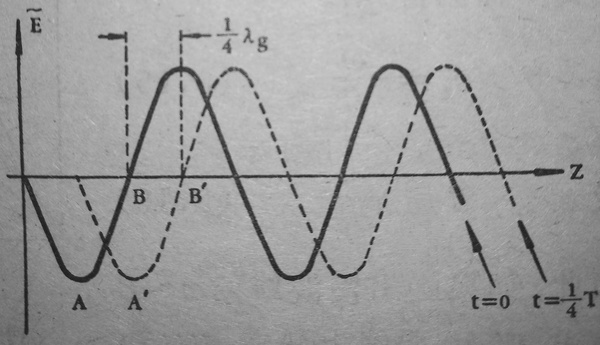
\includegraphics[width=0.65\linewidth]{figure/ch3-3}
	\caption{$ t=0 $和$ t=\frac{1}{4}$时刻,场分量沿$ Z $轴的变化曲线}
	\label{ch3-3}
\end{figure}

\begin{figure}[phtb]
	\centering
	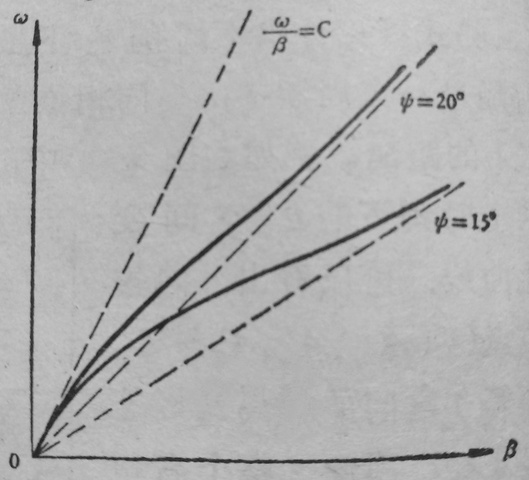
\includegraphics[width=0.65\linewidth]{figure/ch3-4}
	\caption{螺旋线的$ \omega \textasciitilde \beta $曲线}
	\label{ch3-4}
\end{figure}


\begin{figure}[phtb]
	\centering
	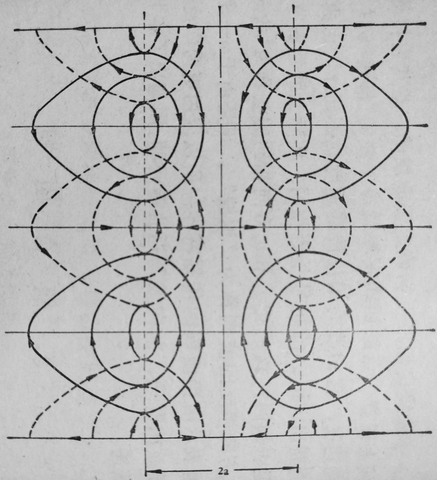
\includegraphics[width=0.65\linewidth]{figure/ch3-5}
	\caption{螺旋线周围电场和磁场分布示意图。实线为电力线,虚线为磁力线。}
	\label{ch3-5}
\end{figure}

\begin{figure}[phtb]
	\centering
	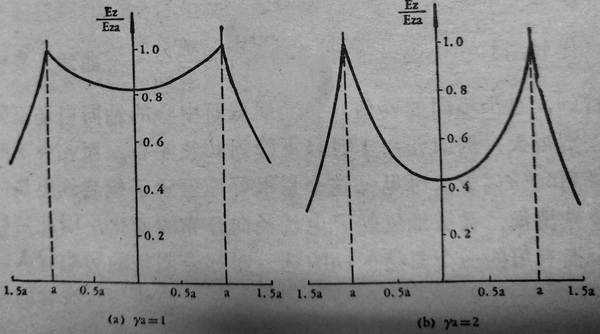
\includegraphics[width=0.65\linewidth]{figure/ch3-6}
	\caption{螺旋线中轴向电场的径向分布示意图}
	\label{ch3-6}
\end{figure}

\begin{figure}[phtb]
	\centering
	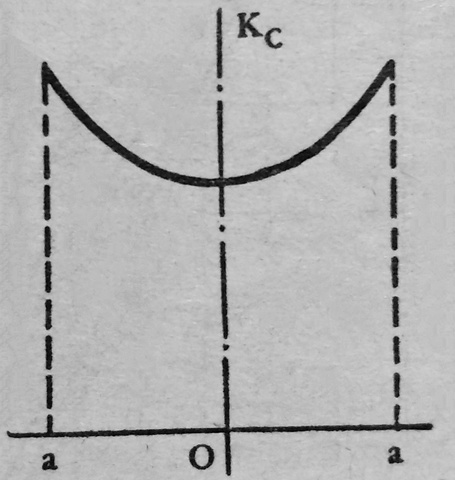
\includegraphics[width=0.65\linewidth]{figure/ch3-7}
	\caption{螺旋线耦合阻抗的径向分布}
	\label{ch3-7}
\end{figure}

\begin{figure}[phtb]
	\centering
	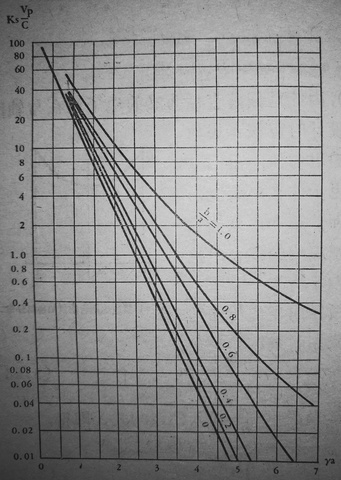
\includegraphics[width=0.65\linewidth]{figure/ch3-8}
	\caption{对于不同的$ \frac{b}{a} $螺旋线耦合阻抗与$ \gamma a $的关系}
	\label{ch3-8}
\end{figure}

\begin{figure}[phtb]
	\centering
	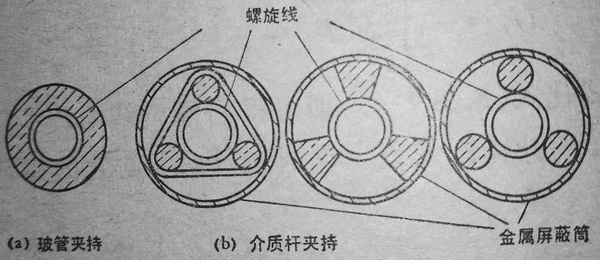
\includegraphics[width=0.65\linewidth]{figure/ch3-9}
	\caption{几种常用的螺旋线加持方法(横截面图)}
	\label{ch3-9}
\end{figure}

\begin{figure}[phtb]
	\centering
	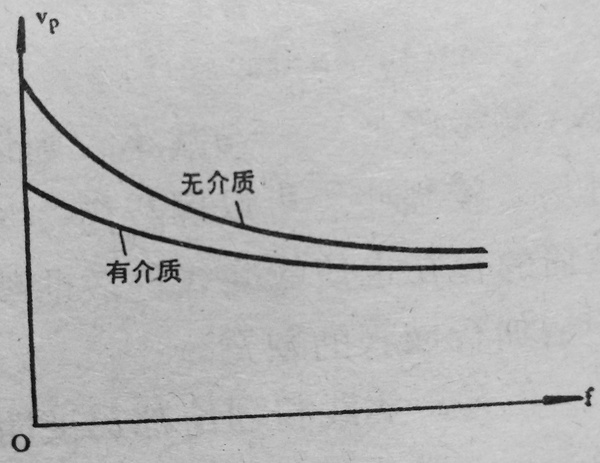
\includegraphics[width=0.65\linewidth]{figure/ch3-10}
	\caption{介质的存在使$ v_p-f $ 曲线变得更平坦}
	\label{ch3-10}
\end{figure}

\begin{figure}[phtb]
	\centering
	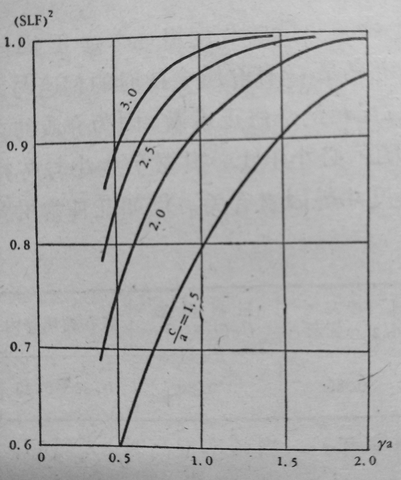
\includegraphics[width=0.65\linewidth]{figure/ch3-11}
	\caption{屏蔽筒加载因子SLF$ ^2 \textasciitilde \gamma a$曲线}
	\label{ch3-11}
\end{figure}